\subsection{Qualitative Comparison Between Analytical and Numerical Solution}

Here it follows a simple and qualitative comparison between the analytical and numerical solution on a single uniform mesh with $N_{el} = 2^{11}$.

\begin{figure}[!ht]
	\centering
	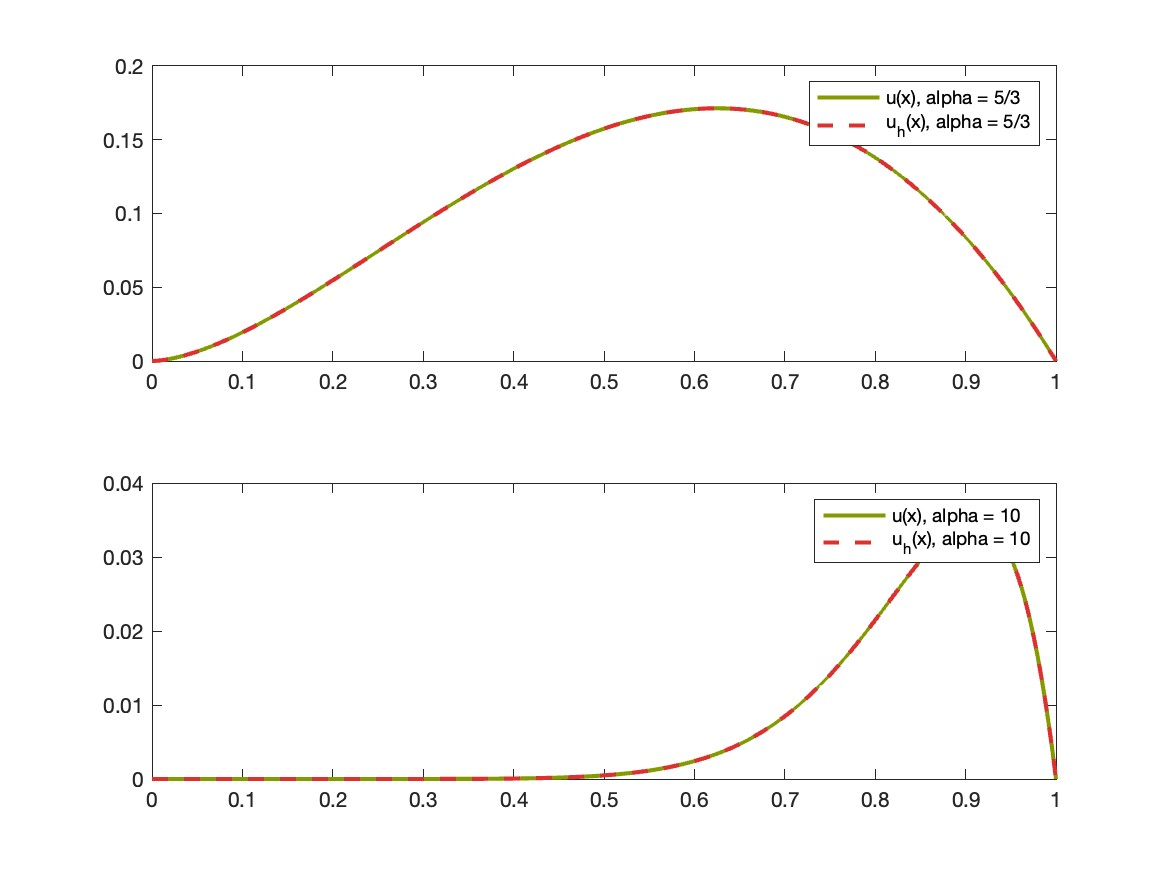
\includegraphics[width=15cm]{graphical.jpg}
	\caption{Qualitative comparison.}
\end{figure}

\subsection{FEM Convergence on Uniform Meshes}

Given what we've said on \nameref{sob_regularity}, and by the following corollary to the \textit{Deny-Lions' Lemma}:

\begin{theorem}[Deny-Lions' corollary]
	Let $u, u_h$ be the solution respectively to the weak formulation of a Poisson problem and its associated order k Lagrangian FEM with shape-regular and quasi-uniform mesh $\Tau_h$. \\ 
	If $u \in H^s(\Omega)$, then $\exists C$ such that:
	\begin{gather}
		|u - u_h|_{1, \Omega} \le C (\max_{K \in \Tau_h} h_K)^{p}|u|_{s+1, \Omega},
	\end{gather}
	with $p = \min(s, k)$.
\end{theorem}

Having defined a 1st-order Lagrangian FEM, we have for both values of $\alpha$ that $p = 1$, so that\footnote{The value of $s$ depends on the value of $\alpha$. We can always choose $s > k$.}:
\begin{gather}
	|u - u_h|_{1, \Omega} \le C (\max_{K \in \Tau_h} h_K)|u|_{s+1, \Omega}.
\end{gather}

By\footnote{For an appropriate choice of $s$.}:
\begin{gather}
	\max_{K \in \Tau_h} h_K = h, \\
	|u|_{s+1, \Omega} < +\infty,
\end{gather}
we have:
\begin{gather}
	|u - u_h|_{1, \Omega} \le C_1 h.
\end{gather}

\begin{figure}[!ht]
	\centering
	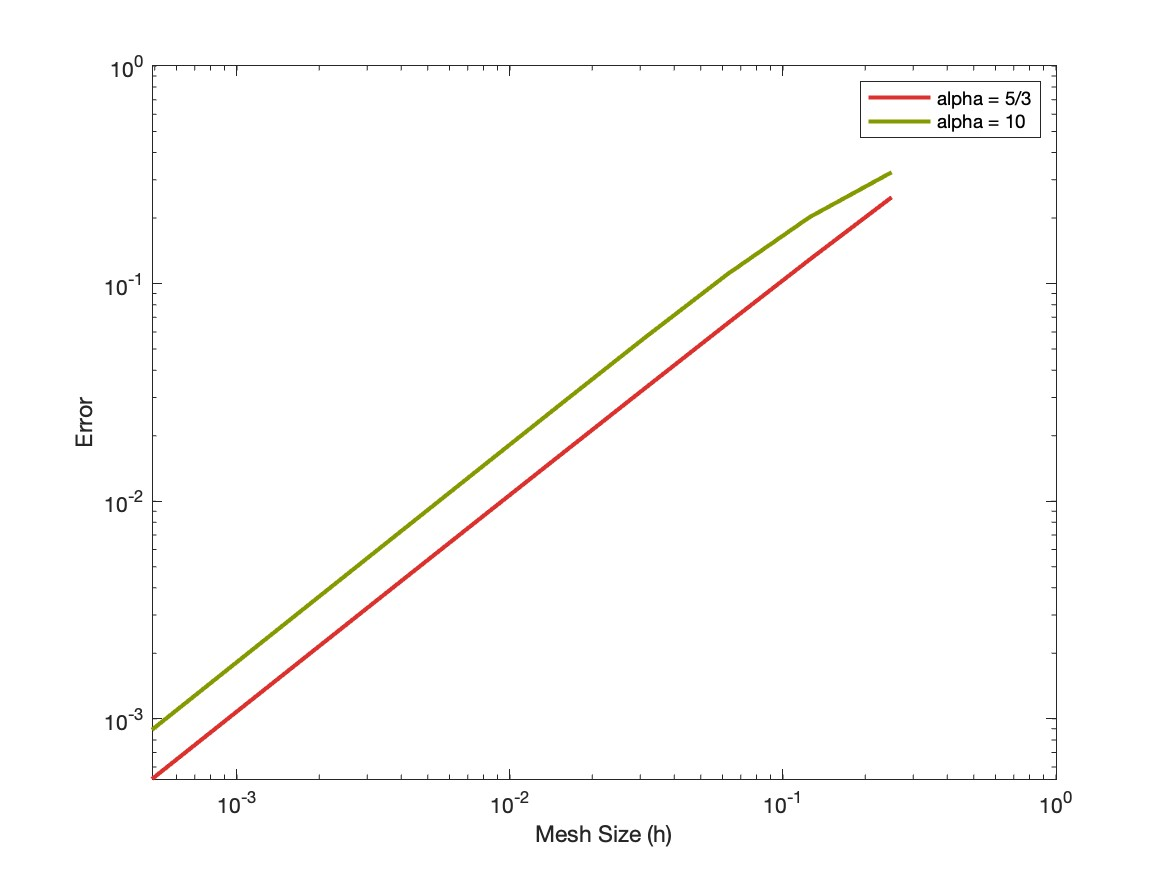
\includegraphics[width=15cm]{errorTrend.jpg}
	\caption{Error trend against mesh size for a sequence of uniform meshes.}
\end{figure}

\newpage
\noindent Moreover a polynomial interpolation returns the following results which confirm the expected error trend on uniform meshes, as they are decreasing slightly slower than linearly\footnote{This is a polynomial interpolation over a loglog relation which we use to return the polynomial order.}.

\lstinputlisting{../results/errorTrend.txt}

\newpage
\subsection{Stiffness Matrix Conditioning}

We want to investigate here the relation between the mesh size and the stiffness matrix' condtion number, expressed as it follows:
\begin{gather}
	\chi(\underline{\underline{A}}) \approx h^{-2}.
\end{gather}

The test is pretty straightforward as it requires to just evaluate the stiffness matrix for different meshes varying just the mesh size.

\begin{figure}[!ht]
	\centering
	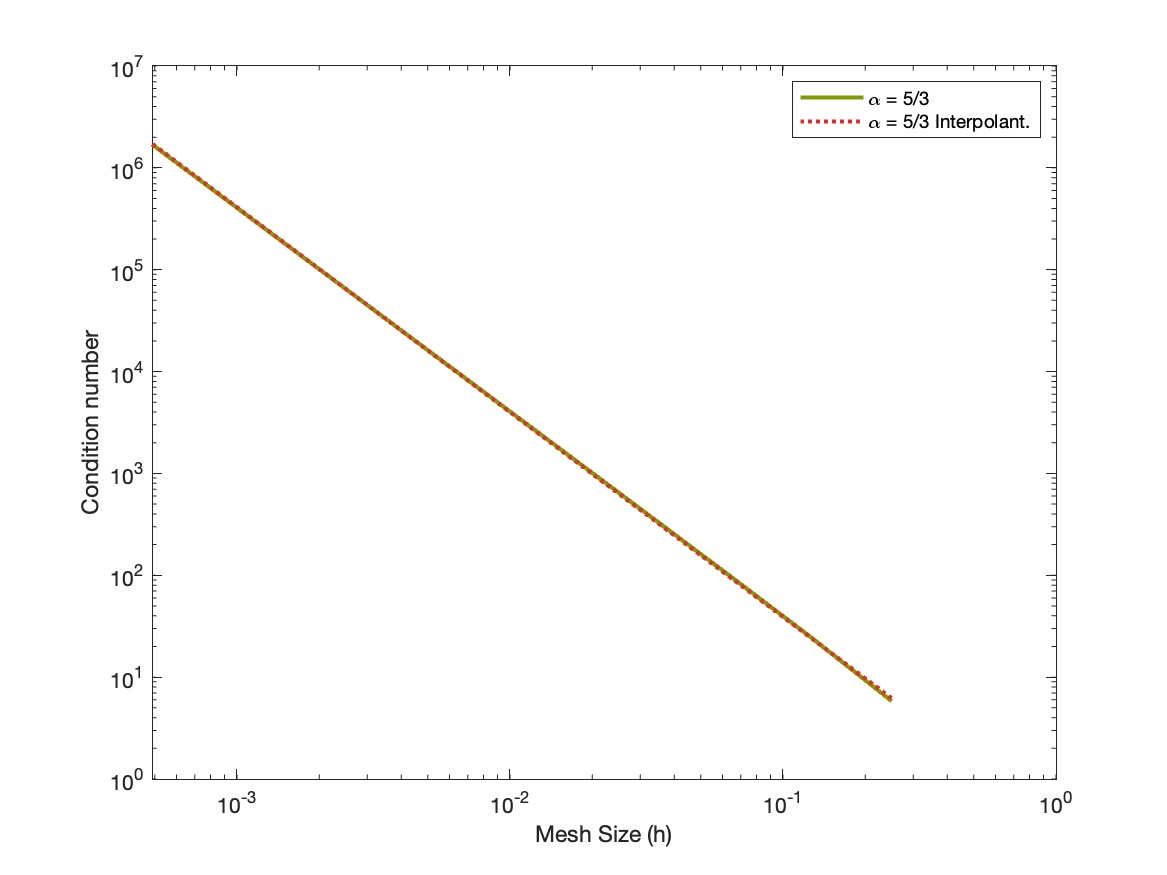
\includegraphics[width=15cm]{condition.jpg}
	\caption{Condition number against mesh size for a sequence of uniform meshes.}
\end{figure}

\newpage
\noindent Moreover a polynomial interpolation returns the following result which confirm the expected condition number trend\footnote{This is a polynomial interpolation over a loglog relation which we use to return the polynomial order.}.

\lstinputlisting{../results/condition.txt}